The calibration constants used in \cref{eq:70}, as mentioned in
\cref{sec:tilecal-calibration}, are determined with the help of several
dedicated calibration systems and runs. Each calibration constant is valid over
a period of time called \gls{iov}. The cell noise can vary over time for several
reasons such as a change in the calibration constants, a variation in the
digital noise or the channel status in a particular run. Sudden variations in
the noise must be checked and understood.

The different TileCal subsystems (laser, CIS, etc.) all use a common software
framework, \gls{tucs}, to perform validity checks on a number of different
studies. To study the stability over time of the updated noise constants, a set
of python scripts was developed by the author of this thesis to expand the TUCS
functionality. These scripts connect to the ATLAS condition database and allow
to visually display the relative change of the cell noise and digital noise
constants, the channel status and the ratio between the cell noise and a
variable called RMS$_\text{eff}$ and defined as:
\begin{equation}
  \label{eq:73}
  \text{RMS}_{\text{eff}} = \sqrt{(1 - R) \sigma_1^2 + R \sigma_2^2}
\end{equation}
where $\sigma_1$, $\sigma_2$ and R are the free parameter in the double Gaussian
model (see Section~\ref{sec:cell-noise}).  The ratio
$\sigma$~/~RMS$_\text{eff}$, where $\sigma$ is the cell noise, can be used to
test the goodness of the double Gaussian model: if $\sigma$~/~RMS$_\text{eff}$
equals one, the double Gaussian well models the noise, if
$\sigma$~/~RMS$_\text{eff}$ $> 1$, it means that there is noise that is not well
described by it.

Figure~\ref{fig:jumps} shows the time evolution plot over the entire reprocessed
period for two representative TileCal cells. This represents the typical
behavior for most cells over the reprocessing period.

In \cref{fig:no_jumps} it can be seen that cell number 2 in the BC layer (BC2)
of the 41st module in the C side of LB (LBC 41) is stable over several pedestal
runs. In Figure~\ref{fig:with_jumps} on the other hand, it is possible to see a
variation in the cell noise and of the $\sigma$~/~RMS$_{\text{eff}}$ without a
corresponding variation in the calibration, in the digital noise constants or in
the channel status. The term \emph{jump} is used in the following to indicate a
variation in the cell noise not compatible with a change in the other
quantities.

\begin{figure}[!h]
  \centering
  \begin{subfigure}[t]{.8\linewidth}
    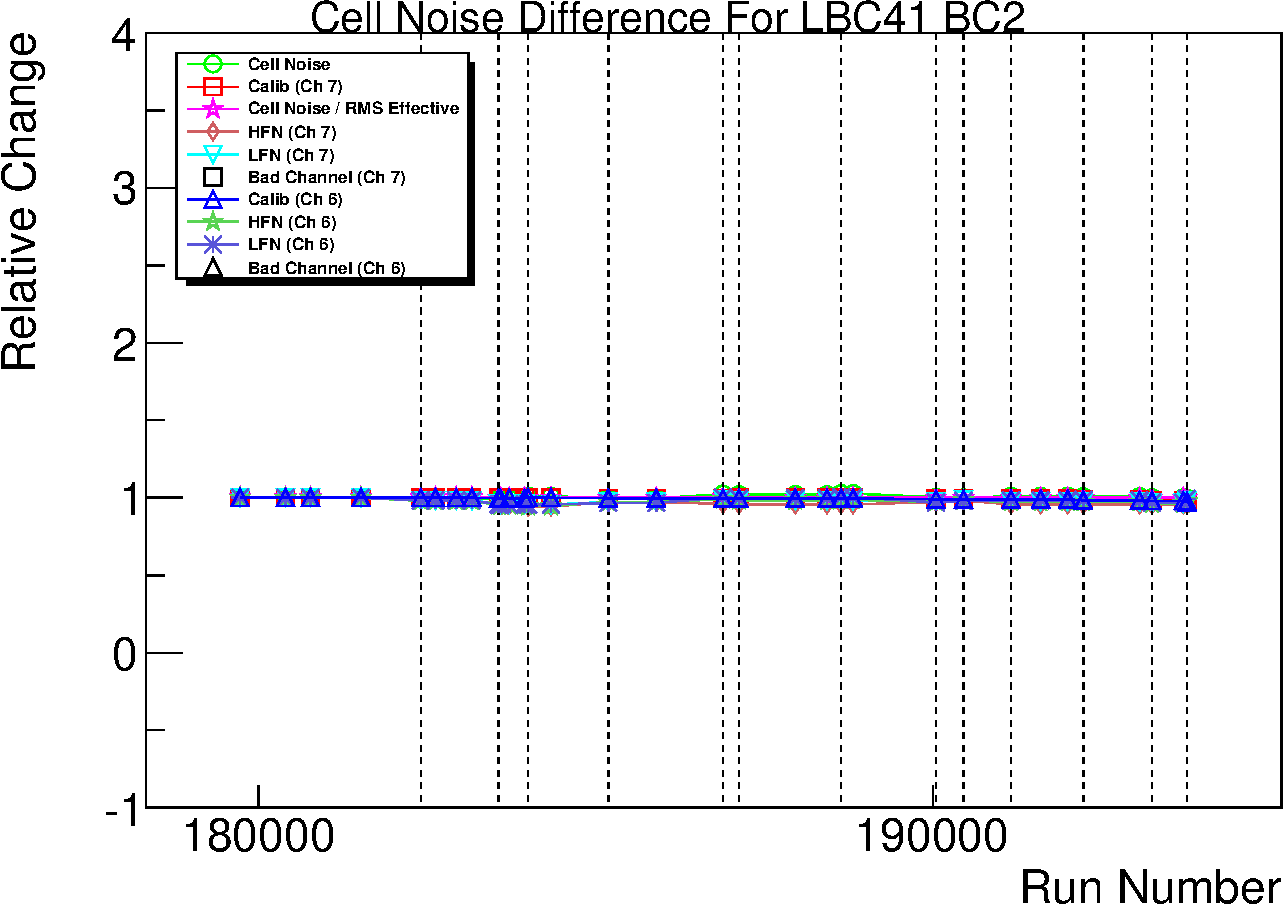
\includegraphics[width=\linewidth]{no_jumps}
    \caption{Control cell with no variation.}
    \label{fig:no_jumps}
  \end{subfigure}
  \begin{subfigure}[t]{.8\linewidth}
    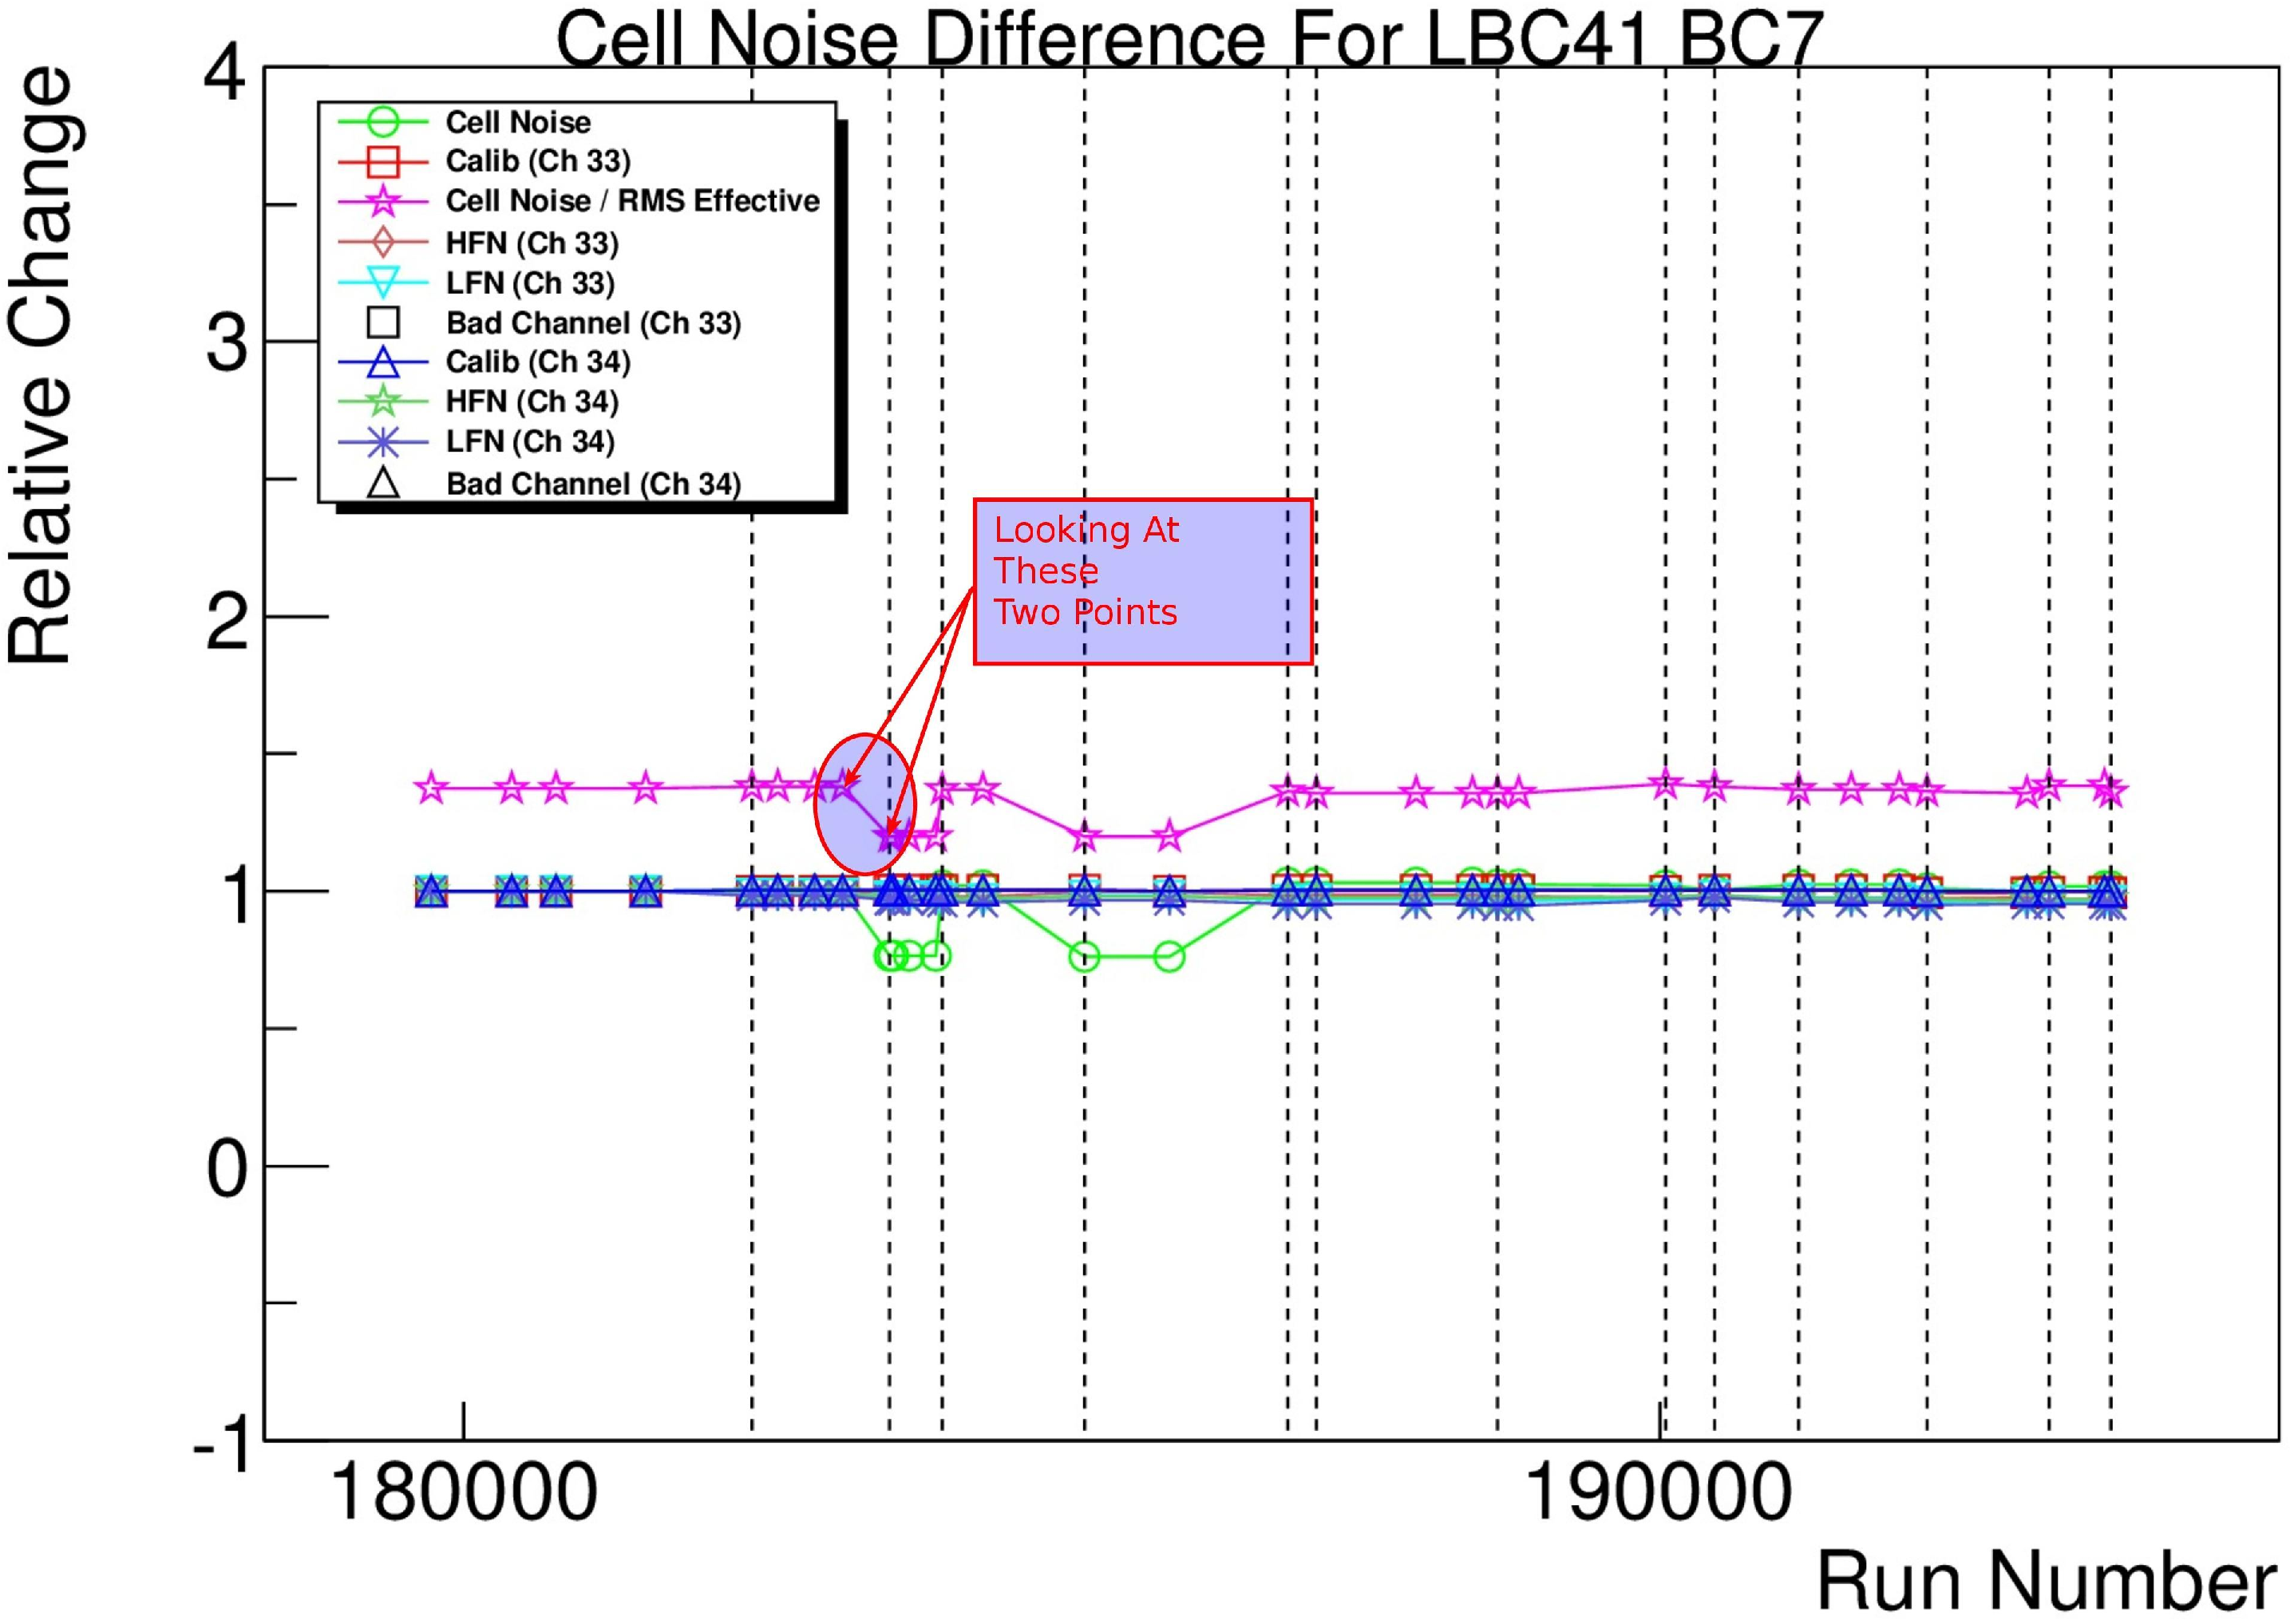
\includegraphics[width=\linewidth]{with_jumps}
    \caption{Cell with a variation.}
    \label{fig:with_jumps}
  \end{subfigure}
  \caption{Time evolution for two different representative cells in the
    calorimeter over the entire reprocessing period. The plot shows the change
    relative to the first run considered for several quantities for different
    IOVs (vertical dashed lines). If a channel is off due to some problems (Bad
    channel), this is reported in the plot with a black square.}
  \label{fig:jumps}
\end{figure}

This problem was investigated by re--performing the pedestal noise
fit\footnote{The standard calibration relies on automated fits performed by the
  ATLAS reconstruction. It was suspected at first that some of these fits were
  failing} manually and recalculating the noise constants focusing on two
specific IOVs, $[183110, 183382[$ (before the jump) and $[183382, 183515[$
(after the jump). Some calorimeter cells without jump were used to validate the
noise constants calculated with the fit and checked against the values stored in
COOL from automated fits performed by the standard ATLAS software.

\cref{fig:no_jump_fit} shows the control cell energy distribution with the
double Gaussian fit superimposed for two runs where the jump was present in
other cells. The results of the fit and the values stored in the COOL database,
both reported in \cref{tab:no_jump_fit}, are in good agreement.
\begin{table}[!h]
  \centering
  \begin{tabular}{r c c}
    \toprule
    \multicolumn{3}{c}{LBC41 BC2 Values Before Jump} \\
    \midrule \midrule
    \quad & Database  & Fit \\
    \midrule
    $\sigma_1$: & 19.97  & $20.08 \pm 0.05$ \\
    $\sigma_2$: & 80.59 & $77.3 \pm 9$ \\
    R\@: & 0.00026  & $0.0003 \pm 0.0012$\\
    \bottomrule
  \end{tabular} \quad
  \begin{tabular}{r c c}
    \toprule
    \multicolumn{3}{c}{LBC41 BC2 Values After Jump} \\
    \midrule \midrule
    \quad & Database & Fit \\
    \midrule
    $\sigma_1$: & 19.94 & $20.05 \pm 0.05$ \\
    $\sigma_2$: & 71.41 & $71.39 \pm 10.51$ \\
    R\@: & 0.00023 & $0.0002 \pm 0.0011$ \\
    \bottomrule
  \end{tabular}
  \caption{The table reports the comparison between the double Gaussian
    parameters stored in the COOL database and those obtained from the
    fit for two different run numbers corresponding to before and after the
    jump for a cell where there is no variation in the cell noise.}
\label{tab:no_jump_fit}
\end{table}

\begin{figure}[!h]
  \centering
  \begin{subfigure}[t]{.8\linewidth}
    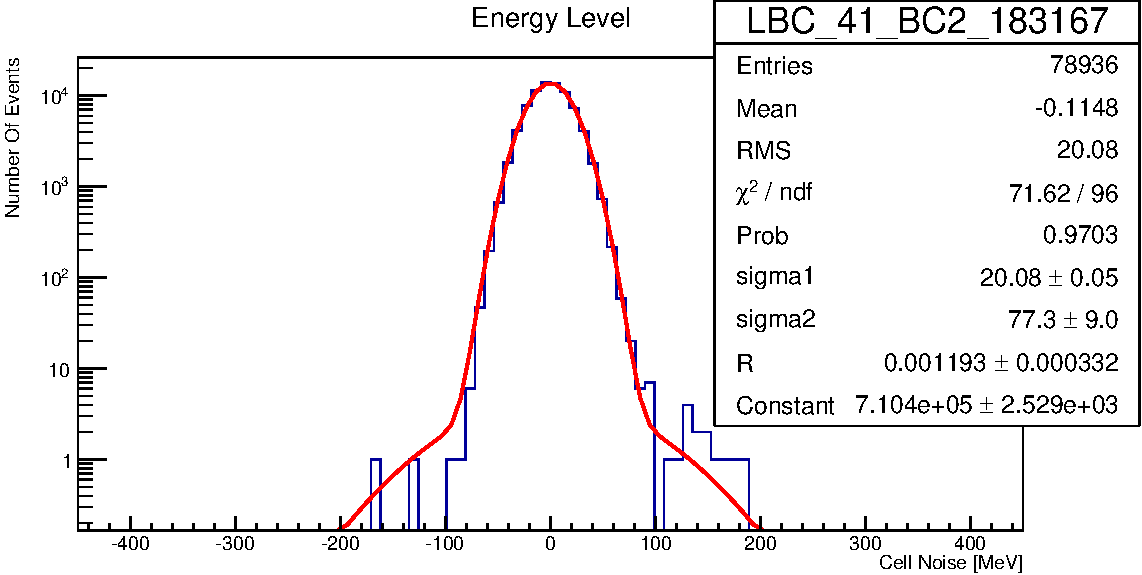
\includegraphics[width=\linewidth]{no_jump_fit_before}
    \caption{Fit before jump.}
    \label{fig:no_jump_fit_before}
  \end{subfigure}
  \begin{subfigure}[t]{.8\linewidth}
    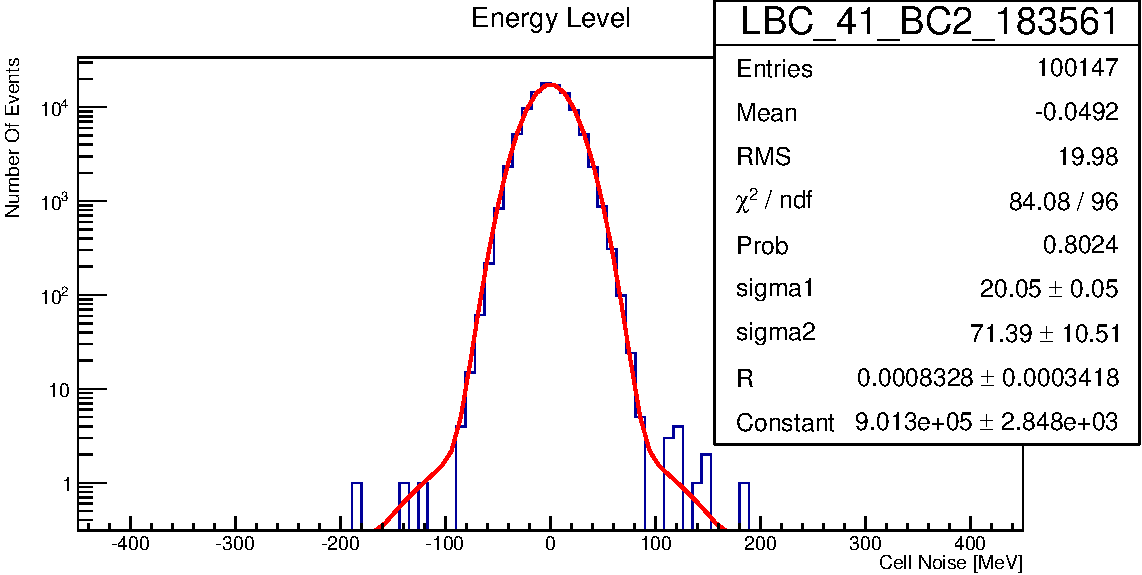
\includegraphics[width=\linewidth]{no_jump_fit_after}
    \caption{Fit after jump.}
    \label{fig:no_jump_fit_after}
  \end{subfigure}
  \caption{Fit of the reconstructed pulse shape on a control cell with no
    variation (jump) in the cell noise.}
  \label{fig:no_jump_fit}
\end{figure}

Moving to the investigation of a cell which exhibits the jump in the time
evolution the seventh cell of the BC layer (BC7) on the C side of the LB
partition of the 41st module (LBC 41) was selected for illustration purposes.
Figure~\ref{fig:jump_fit} shows the energy distribution with the double Gaussian
fit superimposed. The cell had the jump under investigation (see
Figure~\ref{fig:jumps}) and this is reflected in the fit results reported in
\cref{tab:jump_fit} together with the values from the database.
\begin{table}[!h]
  \centering
  \begin{tabular}{r c c}
    \toprule
    \multicolumn{3}{c}{LBC41 BC7 Values Before Jump} \\
    \midrule \midrule
    \quad & Database  & Fit \\
    \midrule
    $\sigma_1$: & 24.25  & $23.56 \pm 0.1$ \\
    $\sigma_2$: & 99.16 & $98.36 \pm 0.9$ \\
    R\@: & 0.037  & $0.042 \pm 0.036$ \\
    \bottomrule
  \end{tabular} \quad
  \begin{tabular}{r c c}
    \toprule
    \multicolumn{3}{c}{LBC41 BC7 Values After Jump} \\
    \midrule \midrule
    \quad & Database & Fit \\
    \midrule
    $\sigma_1$: & 24.42 & $24.4 \pm 0.1$ \\
    $\sigma_2$: & 94.56 & $94.55 \pm 1.34$ \\
    R\@: & 0.014 & $0.014 \pm 0.015$ \\
    \bottomrule
  \end{tabular}
  \caption{The table reports the comparison between the double Gaussian
    parameters stored in the COOL database and those obtained from the
    fit for two different run numbers corresponding to before and after the
    jump for a cell where a variation in the cell noise was spotted.}
  \label{tab:jump_fit}
\end{table}

Also in this case, the noise constants from the fit, are in agreement with those
stored in the COOL database. From this study it was concluded that bad fits
inside the automated ATLAS pedestal and noise reconstruction were not the cause
of the jumps. However, the $\chi^2$ of the distribution imply that the double
Gaussian model is not a good model for the second type of cells.
\begin{figure}[!h]
  \centering
  \begin{subfigure}[t]{.8\linewidth}
    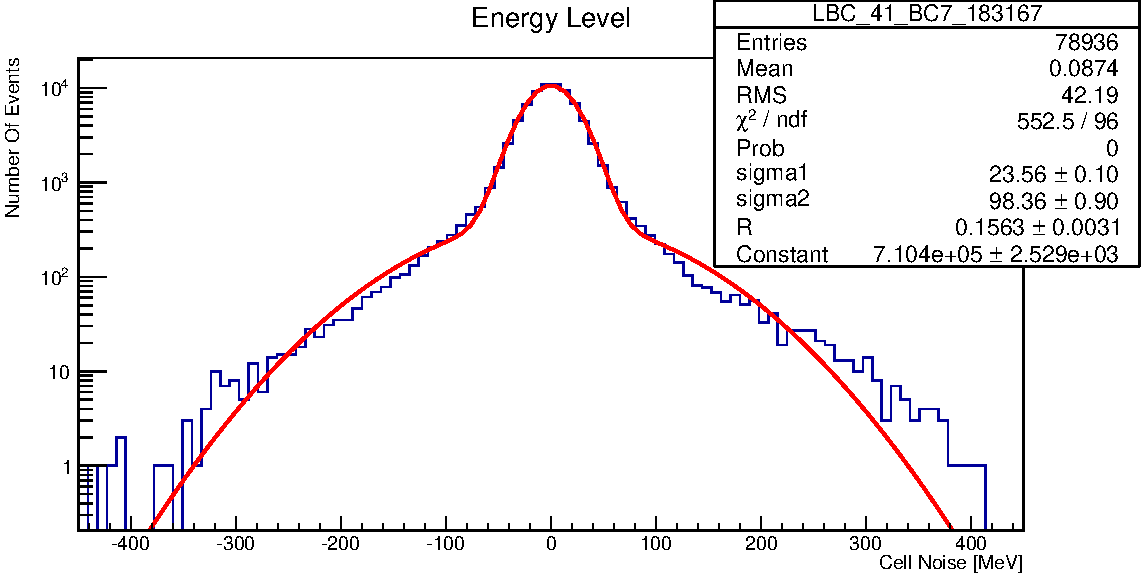
\includegraphics[width=\linewidth]{jump_fit_before}
    \caption{Before jump.}
    \label{fig:jump_fit_before}
  \end{subfigure}

  \begin{subfigure}[t]{.8\linewidth}
    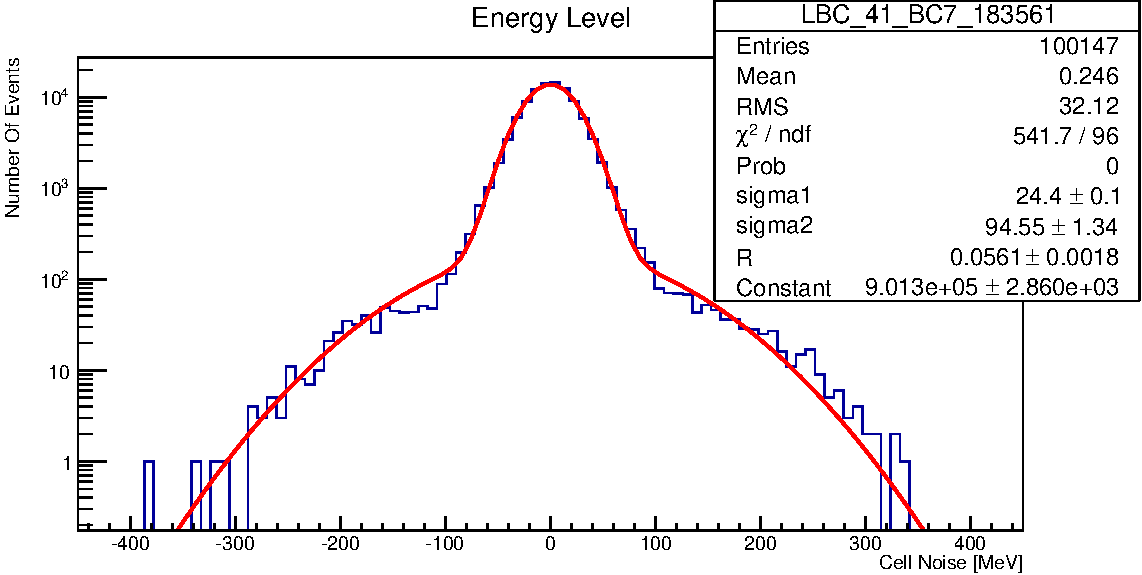
\includegraphics[width=\linewidth]{jump_fit_after}
    \caption{After jump.}
    \label{fig:jump_fit_after}
  \end{subfigure}
  \caption{Fit of the reconstructed pulse shape on a cell with variation (jump)
    in the cell noise non compatible with a change in the calibration, digital
    noise or channel status.}
  \label{fig:jump_fit}
\end{figure}

After further investigations it was discovered that this behavior is caused by
the \gls{tnf}. The electronic noise in nearby channels can be correlated. The
version of low voltage power supplies that were used during the 2011 data taking
lead to significant coherent noise among several channels, particularly those
close to the power supply (see \cref{fig:non_gaussianity}). Coherent noise means
that the signal in several cells can vary coherently and can thus alter the jet
and missing transverse energy reconstruction. In order to remedy this a Tile
Noise Filter was employed. The TNF calculates for each motherboard the pedestal
average:
\begin{equation}
  \label{eq:92}
  d = \frac{\sum_i^N d_i}{N}
\end{equation}
where the index $i$ runs over all the channels belonging to a certain
motherboard, $d_i$ is the $i$--th channel amplitude in ADC counts and $N$ is the
number of channels. Variations in this average baseline can be regarded as an
estimation of the coherent noise and is subtracted from the channel data of each
channel ($d_i - d$) on an event--by--event basis. In order to be able to perform
this noise filter calculation only channels without signal from physics are
taken into account in the sum of \cref{eq:92}.

The cell noise was recalculated without noise filter and the corresponding
distribution re-fitted. \cref{fig:no_filter_fit} show the double Gaussian fit
applied to another cell where the jump was present, in
\cref{fig:d2_fit_before,fig:d2_fit_after} the noise filter is on while in
\cref{fig:d2_fit_before_no_flt,fig:d2_fit_after_no_flt} the TNF was removed. It
can be seen that the fit improves when there is no noise filter. This shows that
the noise jump arises from bad fits when the TNF is somehow malfunctioning and
transforms a double Gaussian distribution into a distribution with more
complicated shape.
\begin{figure}[!h]
  \centering
  \begin{subfigure}[t]{.48\linewidth}
    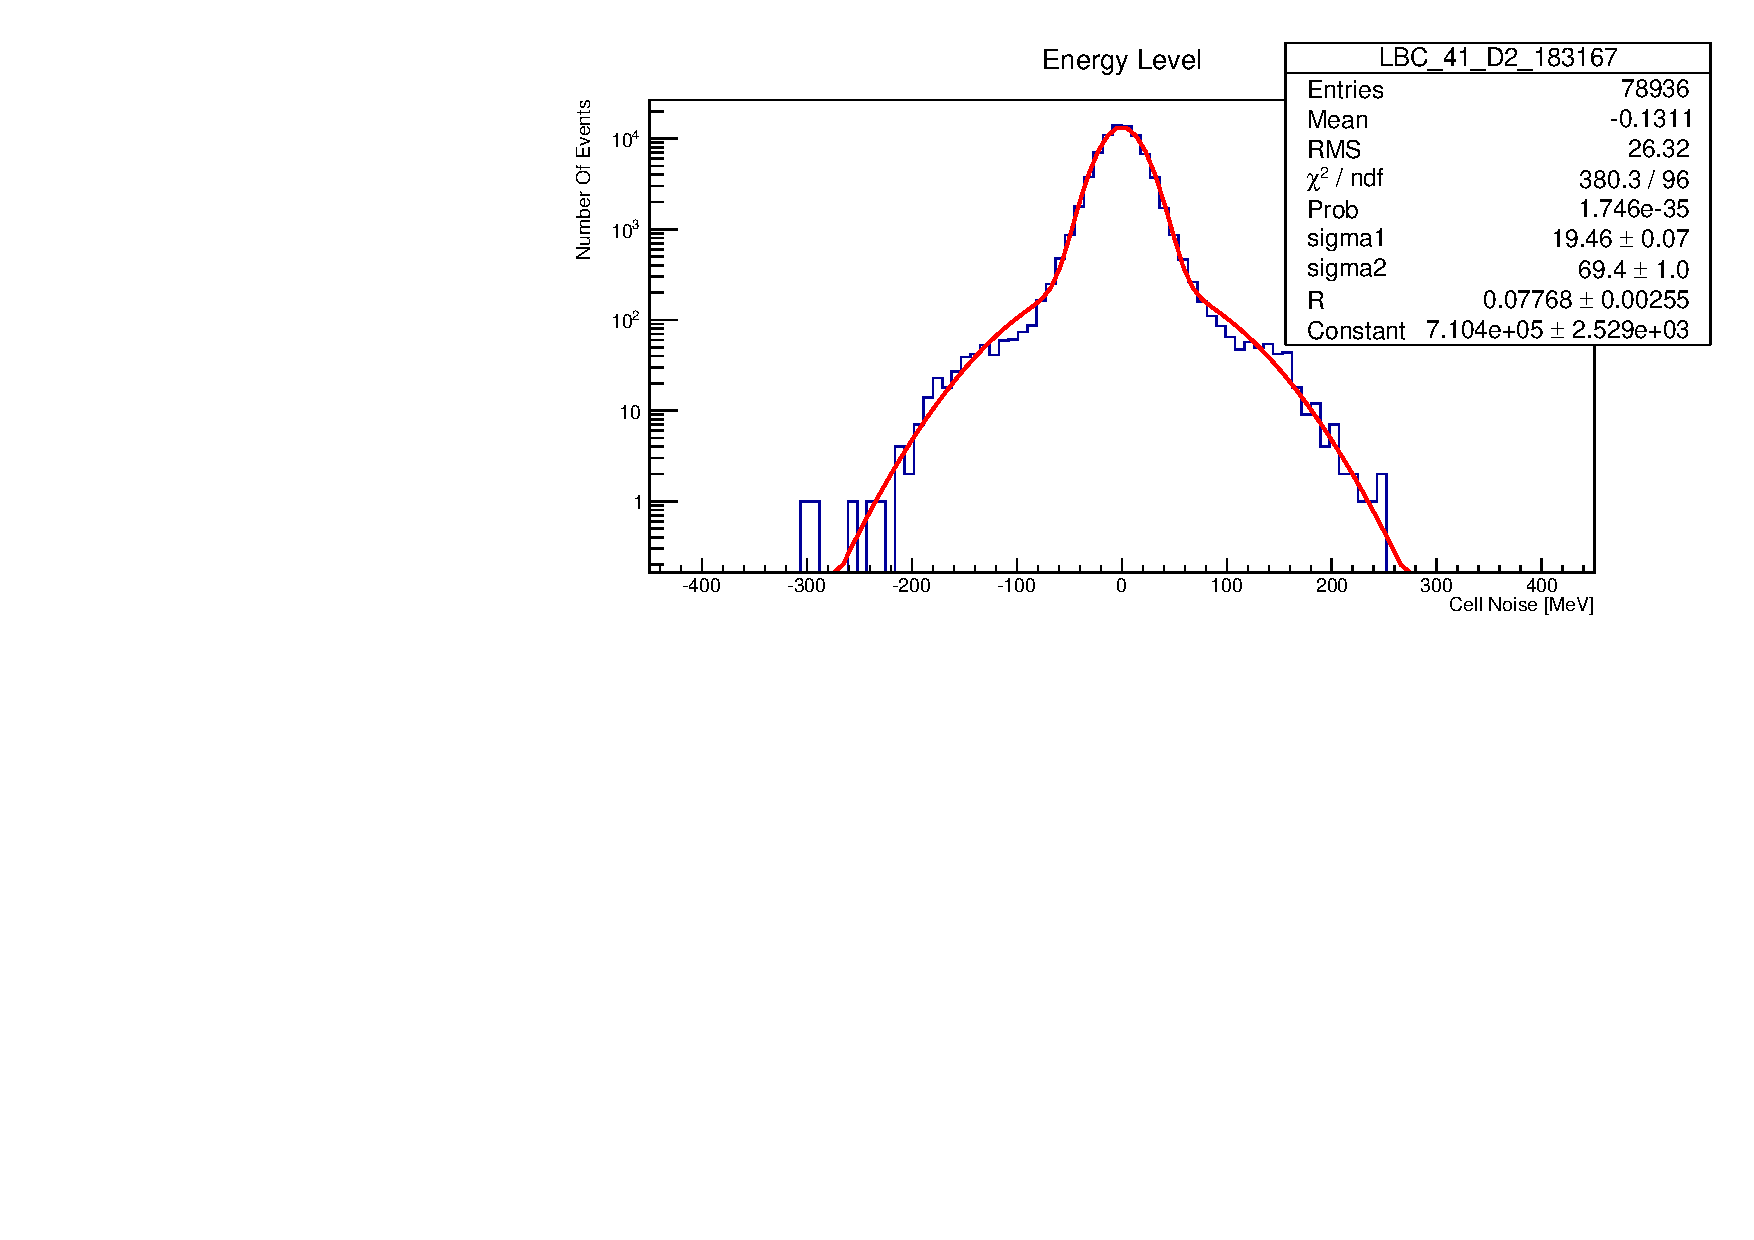
\includegraphics[width=\linewidth]{d2_fit_before}
    \caption{Before jump.}
    \label{fig:d2_fit_before}
  \end{subfigure}
  \begin{subfigure}[t]{.48\linewidth}
    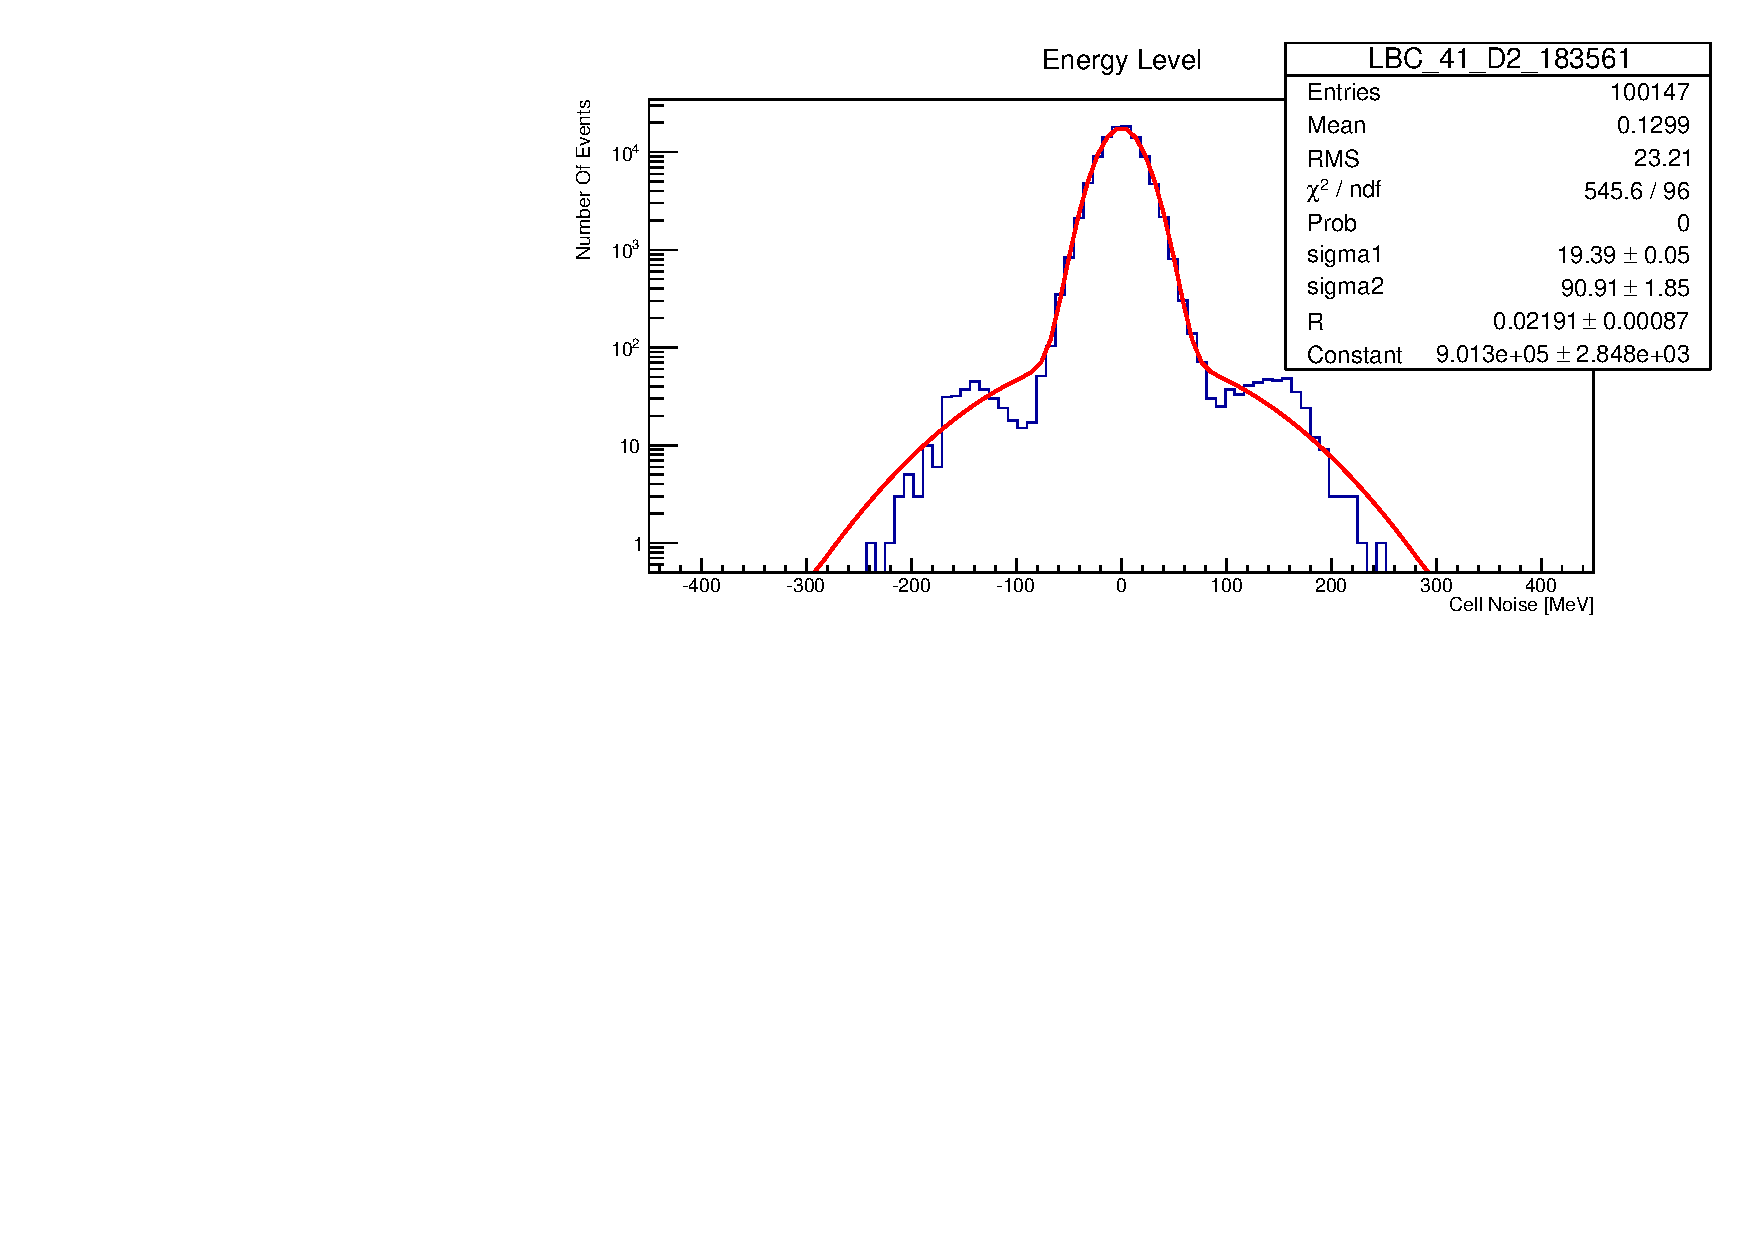
\includegraphics[width=\linewidth]{d2_fit_after}
    \caption{After jump.}
    \label{fig:d2_fit_after}
  \end{subfigure}

  \begin{subfigure}[t]{.48\linewidth}
    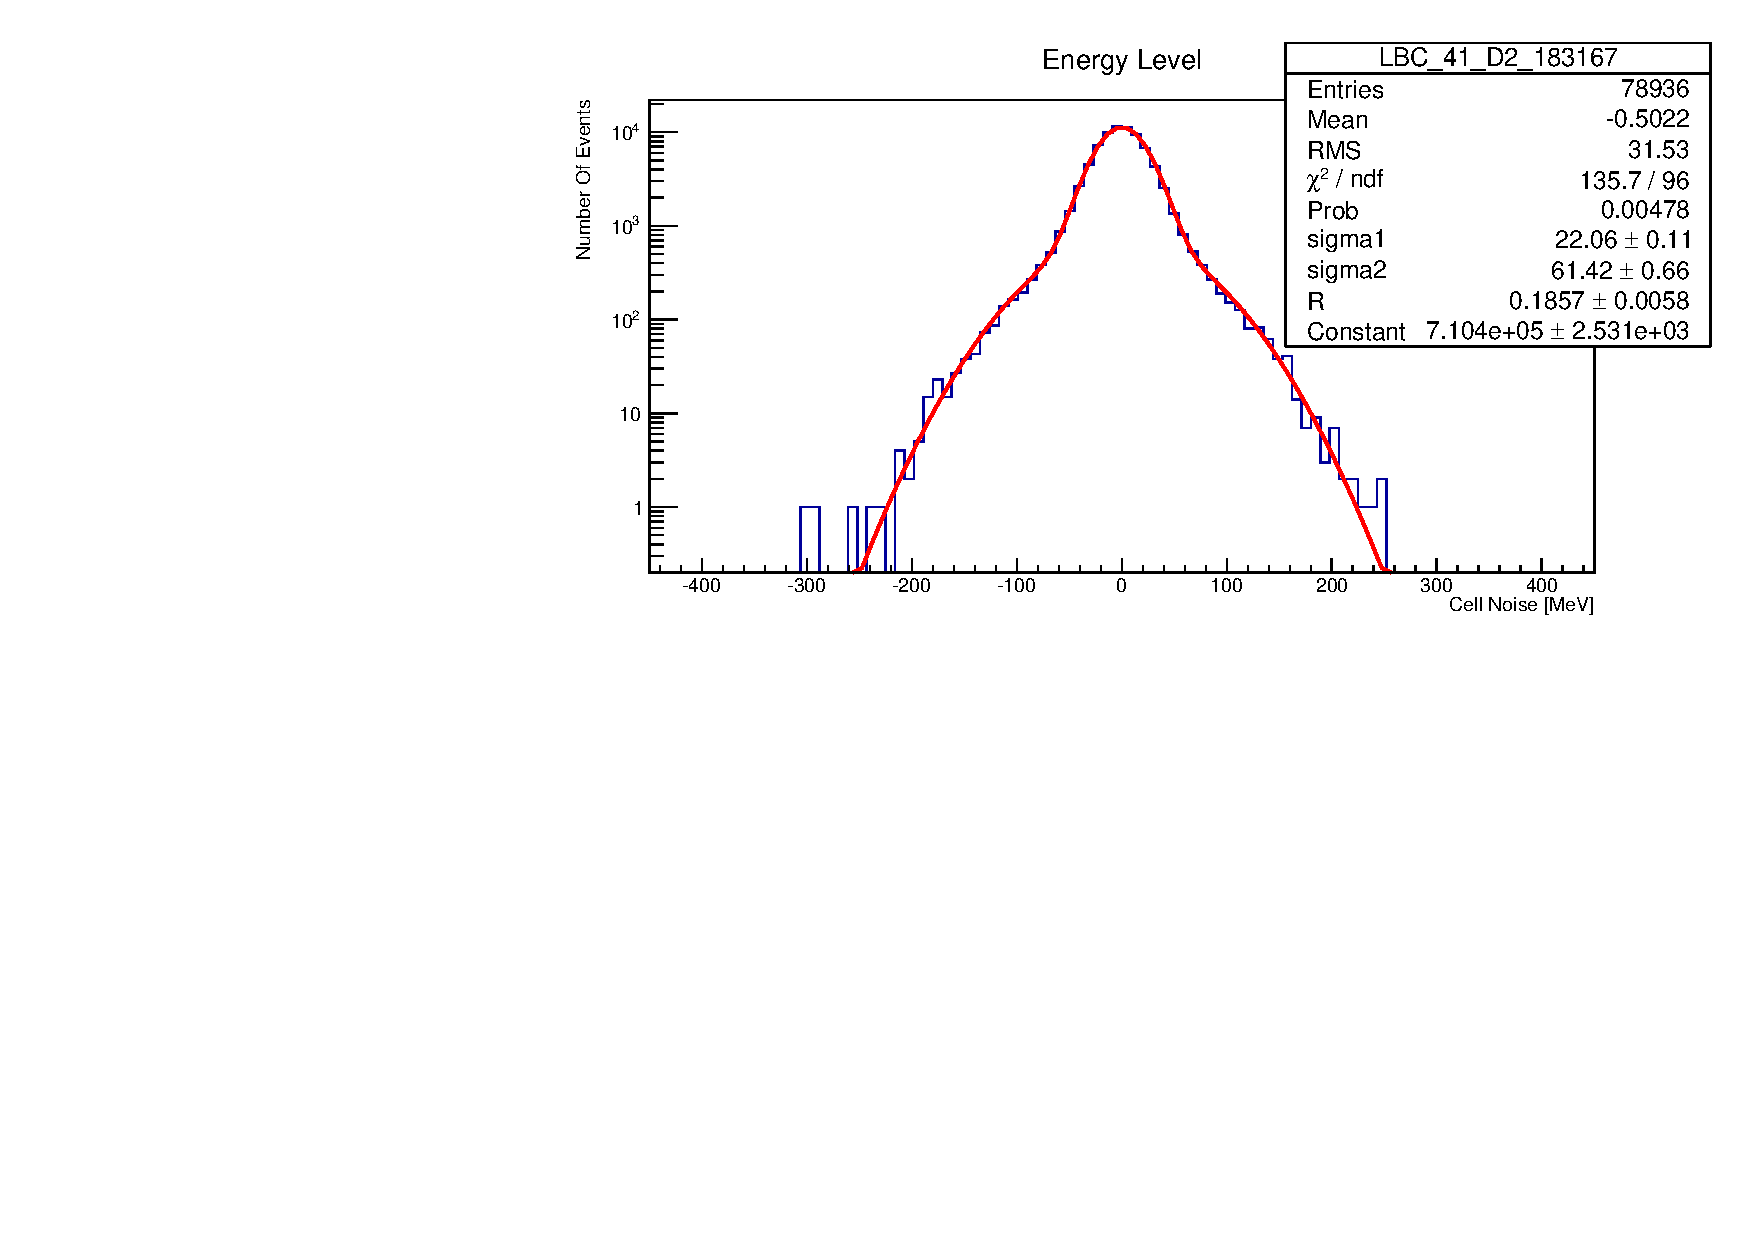
\includegraphics[width=\linewidth]{d2_fit_before_no_flt}
    \caption{Before jump.}
    \label{fig:d2_fit_before_no_flt}
  \end{subfigure}
  \begin{subfigure}[t]{.48\linewidth}
    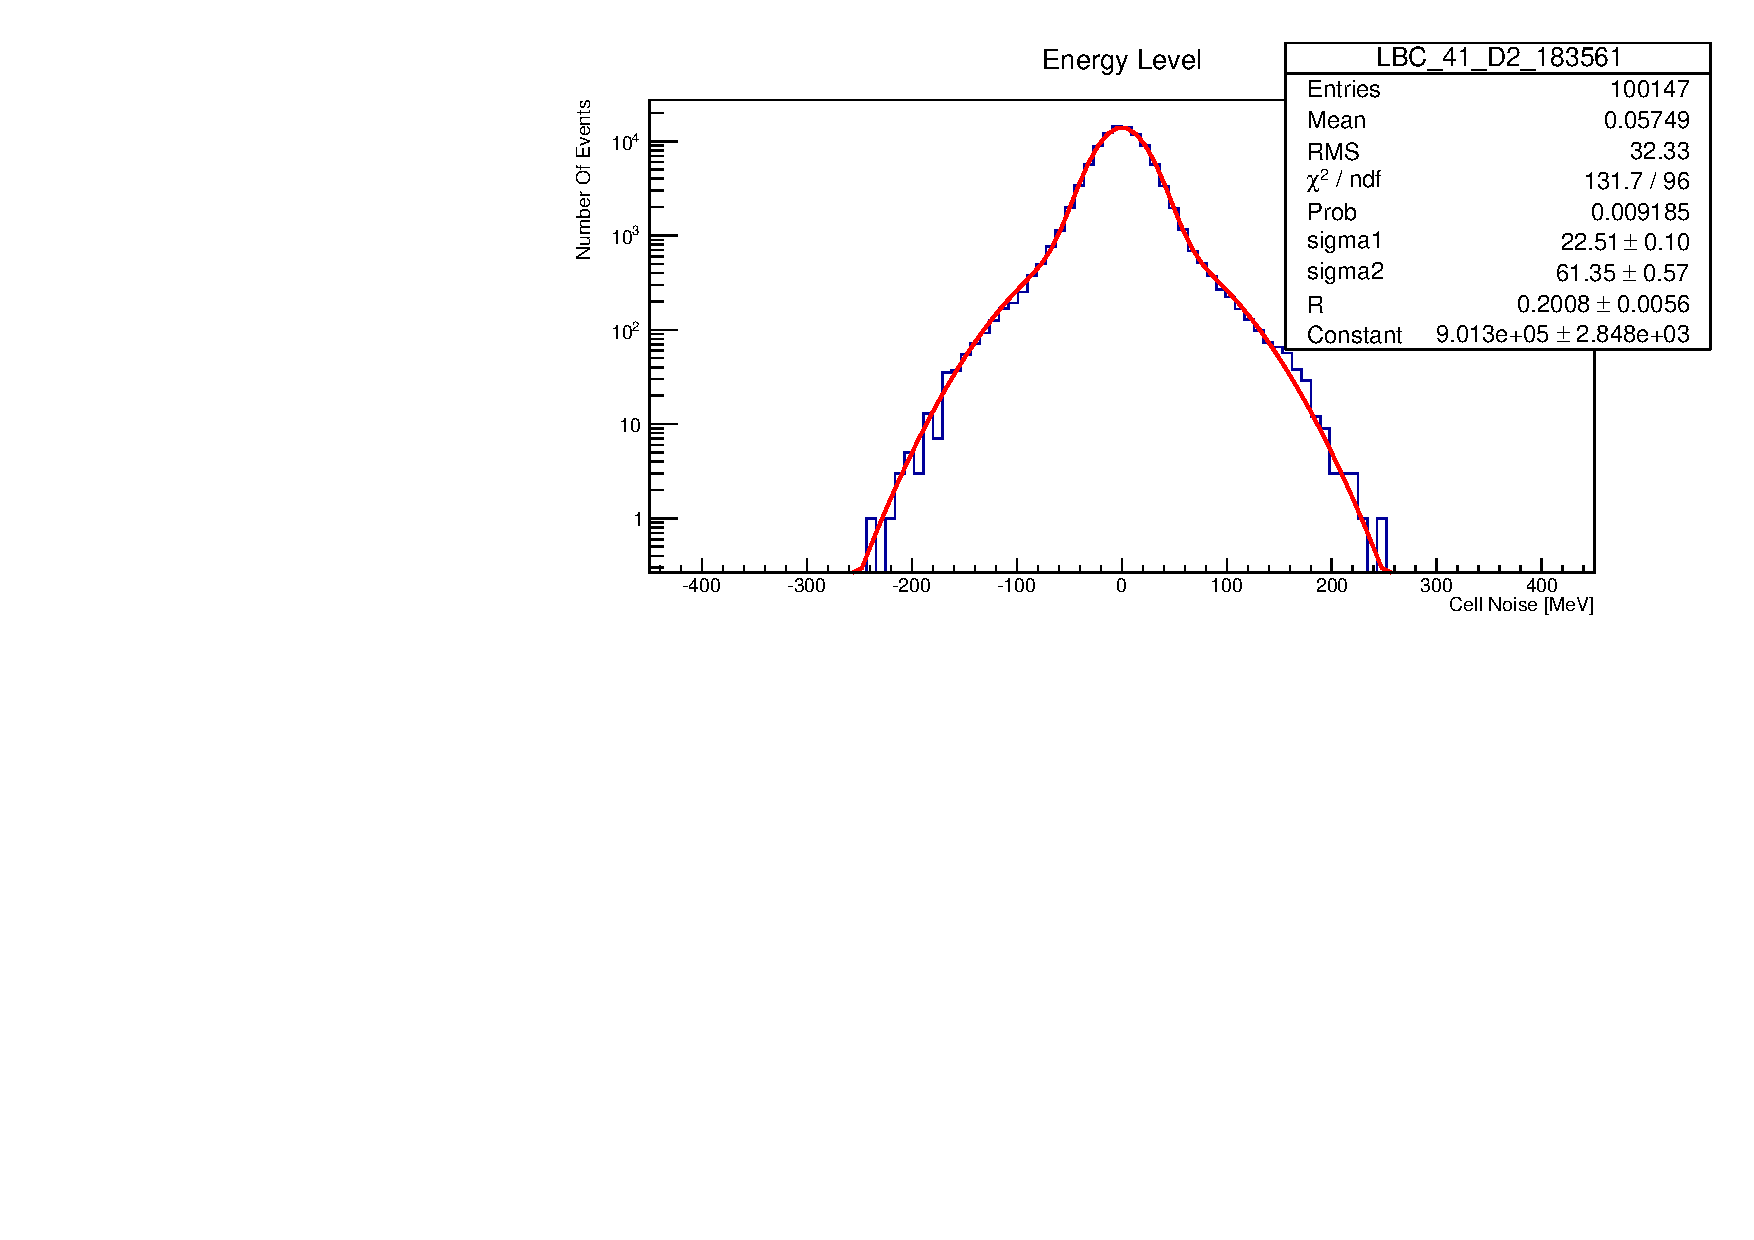
\includegraphics[width=\linewidth]{d2_fit_after_no_flt}
    \caption{After jump.}
    \label{fig:d2_fit_after_no_flt}
  \end{subfigure}
  \caption{Comparison of the reconstructed pulse shape of a cell with the cell
    noise variation without a corresponding variation in he calibration
    constants, digital noise or channel status (jump) with the double Gaussian
    fit superimposed with the noise filter
    (\cref{fig:d2_fit_before,fig:d2_fit_after}) and without noise filter
    (\cref{fig:d2_fit_before_no_flt,fig:d2_fit_after_no_flt}).}
  \label{fig:no_filter_fit}
\end{figure}
%%% Local Variables:
%%% mode: latex
%%% TeX-master: "../search_for_DM_LED_with_ATLAS"
%%% End:
